\documentclass[12pt]{article}

\usepackage[a4paper,margin=2.5cm]{geometry}
\usepackage{amsmath, amssymb, amsthm}
\usepackage{bm}
\usepackage{hyperref}
\usepackage{graphicx}
\usepackage{caption}
\usepackage{listings}
\usepackage{xcolor}
\usepackage{float}
\usepackage{placeins}
\graphicspath{{figures/}}

\lstdefinestyle{code}{
  basicstyle=\ttfamily\small,
  numbers=left,
  numberstyle=\tiny,
  numbersep=8pt,
  keywordstyle=\color{blue},
  commentstyle=\color{teal!70!black},
  stringstyle=\color{orange!70!black},
  showstringspaces=false,
  breaklines=true,
  frame=single,
  framerule=0.3pt,
  rulecolor=\color{black!15}
}
\lstset{style=code}

\title{DBSCAN Clustering Tutorial}
\author{}
\date{\today}

\begin{document}
\maketitle

\section{Introduction}
Density-Based Spatial Clustering of Applications with Noise (DBSCAN) discovers clusters of arbitrary shapes while separating noisy points. By relying on two parameters---the neighborhood radius \(\varepsilon\) and the minimum number of points \(\texttt{minPts}\)---it groups dense regions without predefining the number of clusters. DBSCAN is robust to outliers and especially useful when clusters exhibit varying shapes, though it can struggle when densities differ dramatically between groups.

\section{Theory and Formulas}
\subsection{Neighborhoods and Core Points}
For any point \(p\), the \(\varepsilon\)-neighborhood is defined as
\begin{equation}
\mathcal{N}_\varepsilon(p) = \{ q \mid \lVert p - q \rVert_2 \le \varepsilon \}.
\end{equation}
A point is a \emph{core point} if \(|\mathcal{N}_\varepsilon(p)| \ge \\texttt{minPts}\). A point within a core point's neighborhood but not itself core is termed a \emph{border point}. Points that are neither core nor border are labelled as noise.

\subsection{Density Reachability and Connectivity}
Point \(q\) is directly density reachable from \(p\) if \(p\) is core and \(q \in \mathcal{N}_\varepsilon(p)\). Density reachability is transitive across chains of core points, enabling DBSCAN to form clusters as maximal sets of mutually density-connected points:
\begin{equation}
C = \{ p \mid \exists p_0 \in C_0, p \text{ density reachable from } p_0 \},
\end{equation}
where \(C_0\) contains at least one core point. The algorithm iteratively expands clusters by exploring neighborhoods of core points.

\subsection{Algorithm Outline}
\begin{enumerate}
  \item Standardize features where necessary so that distances are meaningful.
  \item For each unvisited point, query \(\mathcal{N}_\varepsilon(p)\). If \(p\) is not core, mark it as noise temporarily.
  \item If \(p\) is core, create a new cluster and add all points in its neighborhood. Recursively expand by checking neighbors that qualify as core points.
  \item Continue until every point has been assigned to a cluster or marked as noise.
\end{enumerate}
The distance metric influences the notion of density; Euclidean distance is common for numeric features, while cosine or Manhattan distances may be better for sparse or high-dimensional data.

\section{Applications and Tips}
\begin{itemize}
  \item \textbf{Spatial analytics}: DBSCAN detects hot spots such as GPS trajectory stops or crime regions without having to guess cluster counts.
  \item \textbf{Anomaly detection}: Points labelled noise provide a principled way to flag rare events or device faults.
  \item \textbf{Parameter tuning}: Use a k-distance plot (typically with \(k = \texttt{minPts}-1\)) to select \(\varepsilon\); the elbow indicates a stable choice. Start with \(\texttt{minPts} = 2d\) for \(d\) features, and adjust based on noise levels.
  \item \textbf{Preprocessing}: Scale features, remove duplicates, and consider dimensionality reduction when dealing with high-dimensional data so that distance queries remain reliable and efficient.
\end{itemize}

\section{Python Practice}
The accompanying script \texttt{gen\_clustering\_dbscan\_figures.py} generates synthetic two-dimensional data with three dense regions and peripheral noise. It fits DBSCAN for a range of \(\varepsilon\) values, stores an illustrative clustering, and produces an ordered k-distance curve for diagnosing parameter choices.
\begin{lstlisting}[language=Python,caption={Excerpt from gen_clustering_dbscan_figures.py}]
from sklearn.cluster import DBSCAN
from sklearn.neighbors import NearestNeighbors

# Fit DBSCAN with Euclidean distance
dbscan = DBSCAN(eps=0.35, min_samples=5, metric="euclidean")
dbscan.fit(points)
labels = dbscan.labels_

# Compute ordered distances to the k-th nearest neighbor
neighbors = NearestNeighbors(n_neighbors=5)
neighbors.fit(points)
dists, _ = neighbors.kneighbors(points)
k_distance = np.sort(dists[:, -1])
\end{lstlisting}

\section{Result}
\begin{figure}[H]
  \centering
  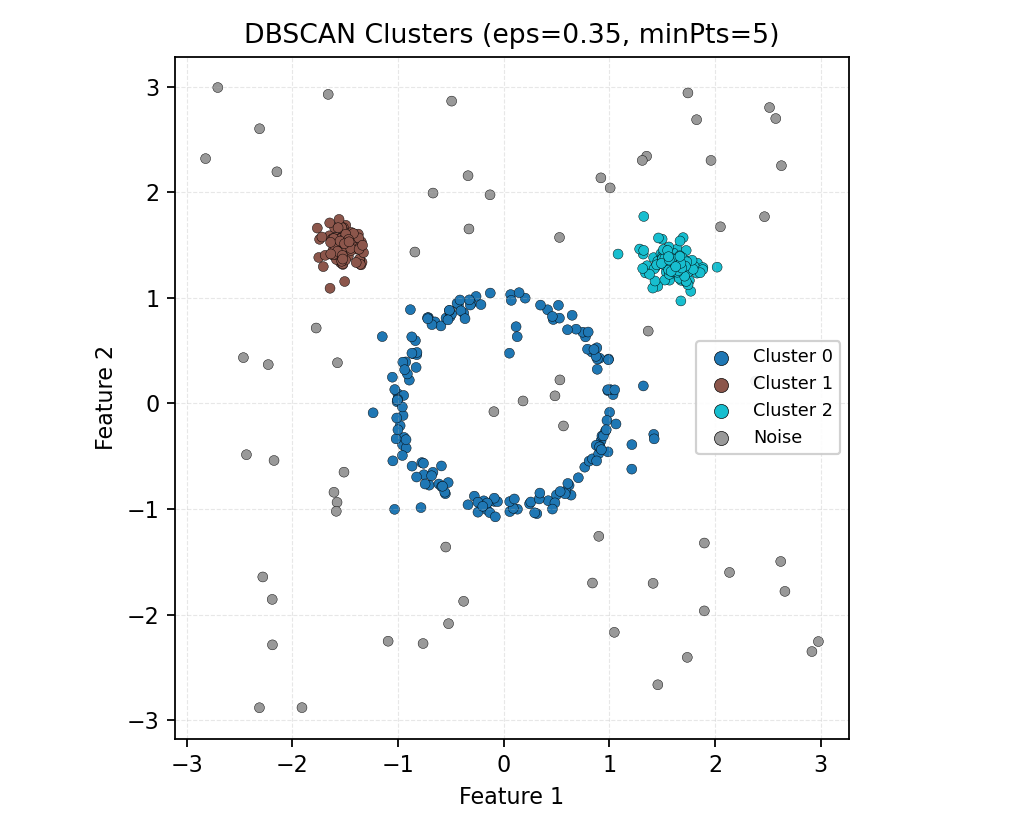
\includegraphics[width=0.8\linewidth]{dbscan_clusters.png}
  \caption{DBSCAN clusters on synthetic data with noise (\(\varepsilon=0.35, \texttt{minPts}=5\))}
  \label{fig:dbscan_clusters}
\end{figure}

\begin{figure}[H]
  \centering
  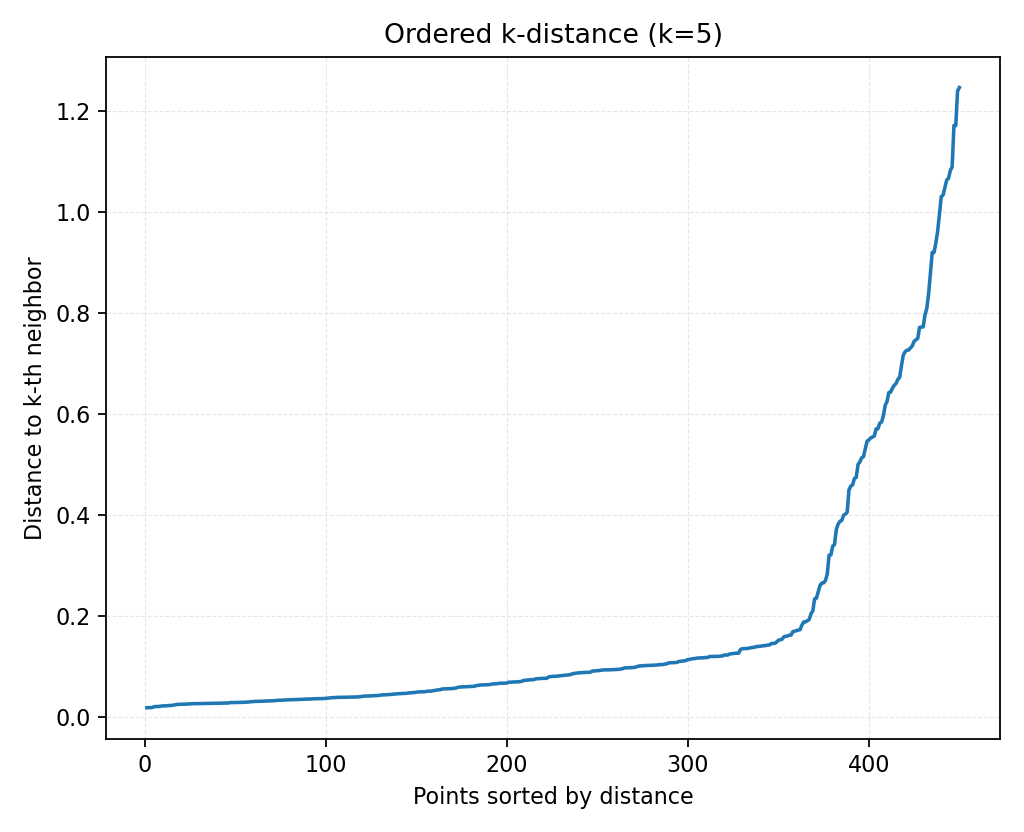
\includegraphics[width=0.8\linewidth]{dbscan_k_distance.png}
  \caption{Ordered k-distance plot highlighting the elbow near \(\varepsilon=0.35\)}
  \label{fig:dbscan_k_distance}
\end{figure}

\FloatBarrier
\section{Summary}
DBSCAN excels at uncovering arbitrarily shaped clusters without specifying their count while labelling sparse regions as noise. Effective use hinges on meaningful distance metrics, thoughtful scaling, and data-driven selection of \(\varepsilon\) and \texttt{minPts}. The synthetic example demonstrates how clustering output and k-distance diagnostics work together to justify parameter choices.

\end{document}
